\documentclass[a4paper,10pt]{article}

\usepackage{tikz}
\usepackage{fullpage}
\usepackage{amsmath,amsthm,amsfonts,amssymb,amscd}
\usepackage{mathtools}
\usepackage{colortbl}
\usepackage{xcolor}
\usepackage{graphicx}
\usepackage{titlesec}
\usepackage{xepersian}
\usepackage{multirow}
\usepackage{enumitem} % for alphabetic item labels

% ---------------------------
%      Dark Theme Setup
% ---------------------------
\definecolor{CustomBackground}{HTML}{1C1C1C}  % Dark background
\pagecolor{CustomBackground}
\color{white}

% ---------------------------
%        Font Setup
% ---------------------------
\settextfont{Vazir.ttf}[
    BoldFont = Vazir-Bold.ttf,
    Path = fonts/
]
\setlatintextfont{Vazir.ttf}[
    BoldFont = Vazir-Bold.ttf,
    Path = fonts/
]

% ---------------------------
%     Custom Adjustments
% ---------------------------
\renewcommand{\baselinestretch}{1.2}
\renewcommand{\thesection}{\arabic{section}}

% User-defined commands for homework info (adjust as needed)
\newcommand{\HomeworkNumber}{2}
\newcommand{\HomeworkDeadline}{1404/7/26}
\newcommand{\id}{\texttt{\detokenize{@reza051taji}}}

\begin{document}

% ---------------------------------
%           Front Page
% ---------------------------------
\begin{titlepage}
    \begin{center}
        \vspace*{1cm}
        % Bigger Logo
        
\includegraphics[scale=1.1]{assets/fum-logo.png}\\[1cm]

        {\Huge \bfseries مبانی و کاربردهای هوش مصنوعی}\\[0.5cm]
        {\Large دانشگاه فردوسی مشهد}\\[0.3cm]
        {\Large گروه مهندسی کامپیوتر}\\[0.5cm]
        {\normalsize دکتر هراتی}\\[2cm]

        {\Huge \bfseries تمرین \HomeworkNumber}\\[0.5cm]
        {\Large مهلت تحویل: \HomeworkDeadline}\\[2.5cm]

        \Large مسئول تمرین: \id
    \end{center}
\end{titlepage}

% ---------------------------------
%          Instructions
% ---------------------------------
\clearpage
\section*{دستورالعمل‌ها}

دانشجویان محترم لطفا به موارد زیر توجه فرمایید:
\begin{itemize}
\itemsep0em
\item
	تحويل تمرين‌ها فقط از طريق سامانه  آموزش مجازی دانشگاه امکان‌‌پذیر است.
\item 
	تمرین‌ها باید دست نویس، خوانا و با استفاده از خودکار آبی یا مشکی و یا به صورت دیجیتالی با استفاده از قلم نوری نوشته شوند. 
\item
از تمرین‌های حل شده دیگران و هوش مصنوعی استفاده نکنید. پیامد‌های این کار با دانشجو می‌باشد. 
\item
	نوشتن جواب آخر به تنهايى نمره‌ای نداشته و تمام مراحل حل، مشمول نمره می‌باشد.
\item 
	به دلیل موعد از پیش تعیین شده تمرین‌ها و برنامه درسی، امکان تمدید تمرین وجود ندارد. همچنین بدیهی است که ارسال تمرین پس از موعد تعیین شده نمره‌ای نخواهد داشت.
	
\item نحوه نام‌گذاری فایل پاسخ باید مطابق جدول \ref{tab:file_format}
و به شکل pdf باشد.

\begin{table}[h]
	\centering
	\begin{tabular}{|c|c|}
		\hline
		\textbf{Format} & \texttt{StudentID-Full\_Name-\#HwNo.pdf} \\
		\hline
		\textbf{Example} & \texttt{9876543210-Alan\_Turing-\#02.pdf} \\
		\hline
	\end{tabular}
	\caption{شیوه نام‌گذاری فایل‌ها}
	\label{tab:file_format}
\end{table}
    
    
\end{itemize}
\rule{\linewidth}{0.4pt}

% -------------------------
%        Questions
% -------------------------

\section{سوال اول}
درستی یا نادرستی عبارات زیر را با ذکر دلیل (حداکثر دو خط) مشخص نمایید.
\begin{enumerate}[label=\alph*-]
    \item تابع هیوریستیک $h(n)=0$ هیوریستیکی قابل قبول برای تمام مسائل است.
    \item روش‌های مبتنی بر جستجوی درخت (Tree-Search) تنها برای فضای حالت با ساختار درخت به کار میروند.
    \item الگوریتم IDA* یک روش جستجوی اول بهترین (Best-First) نیست.
    \item اگر تابع ابتکاری $h_1$ به ازای هر گره تخمین بیشتری از $h_2$ بزند، $h_1$ تابع بهتری نسبت به $h_2$ می‌باشد.
    \item هر پاسخ بهینه در مسئلۀ اصلی، یک پاسخ بهینه برای Problem Relaxed است.
\end{enumerate}

% اگر تصویر مرتبط دارید، این خط را آنکامنت کنید و نام فایل را در assets/ قرار دهید:
% \begin{center}
%   \includegraphics[width=0.6\textwidth]{assets/q1-image.png}
% \end{center}

\bigskip
\rule{\linewidth}{0.4pt}

\section{سوال دوم}
گزاره‌های درست را اثبات و گزاره‌های نادرست را با آوردن مثال نقض رد کنید.
\begin{enumerate}[label=\alph*-]
    \item اگر تابع هیوریستیک تابع ثابت باشد، الگوریتم A* بهینه است.
    \item هر تابع هیوریستیک قابل قبول (Admissible) یکنواخت (Consistent) نیز است.
    \item الگوریتم IDA* در بدترین حالت به اندازه فضای حالاتش Iteration دارد.
    \item فضای حالات در مسئلۀ اصلی، زیرمجموعۀ Problem Relaxed شده است.
\end{enumerate}

% تصویر (در صورت وجود):
% \begin{center}
%   \includegraphics[width=0.6\textwidth]{assets/q2-image.png}
% \end{center}

\bigskip
\rule{\linewidth}{0.4pt}

\section{سوال سوم}
دو اصطلاح Measure Performance و Function Evaluation را تعریف کرده و تفاوت آنها را در ارتباط با عامل (Agent) را مشخص کنید.

\bigskip
\rule{\linewidth}{0.4pt}

\section{سوال چهارم}
تفاوت دو روش جستجوی درخت (Tree-Search) و جستجوی گراف (Graph-Search) چیست؟ با ذکر مثال توضیح دهید که اگر در روش جستجوی گراف، تابع هیوریستیک یکنواخت نباشد چه مشکلی بوجود می‌آید؟

\bigskip
\rule{\linewidth}{0.4pt}

\section{سوال پنجم}
مشکل اصلی الگوریتم A* چیست؟ توضیح دهید هر یک از سه الگوریتم IDA* و RBFS و MA* چگونه این مشکل را رفع می‌کنند؟ سه الگوریتم را از نظر پیچیدگی حافظه با هم مقایسه کنید. مسئله زیر را با استفاده از الگوریتم RBFS حل کنید.

\begin{itemize}
    \item عامل می‌خواهد از خانه آغاز S به خانه پایان G برود.
    \item عامل در هر گام تنها یک خانه به یکی از جهت‌های بالا، پایین، چپ یا راست جابجا می‌شود.
    \item هزینه هر گام 1 واحد است.
    \item عامل در هر مسیر خود، از یک خانه حداکثر یک‌بار می‌گذرد؛ مثلاً اگر از C2 به C3 برود، در ادامۀ آن مسیر به C2 باز نمی‌گردد.
    \item از هیوریستیک فاصله منهتن استفاده کنید.
    \item هر گره وضعیت را با شماره خانه مشخص کنید؛ برای مثال گره ابتدایی C2 است.
    \item رسم درخت برای هر مرحله تا قبل از Backtracking و نوشتن مقادیر \texttt{f-value} و \texttt{best-alternative} برای گره‌ها لازم است.
\end{itemize}

% اگر پلان یا نقشه‌ی مسئله دارید، اینجا قرار دهید:
\begin{center}
  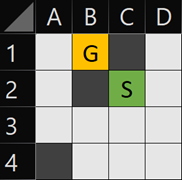
\includegraphics[width=0.3\textwidth]{assets/q5-map.png}
\end{center}

\bigskip
\rule{\linewidth}{0.4pt}

\section{سوال ششم}
برای طراحی تابع هیوریستیک به روش زیرمسئله (Subproblem) برای مسئله پازل 8، دو زیرمسئلۀ بصورت زیر بیان شده‌اند. برای هر یک توضیح دهید که دو مقدار هیوریستیک چگونه با یکدیگر ترکیب شوند تا هیوریستیک مسئلۀ اصلی قابل قبول باشد؟ (دو روش ترکیب متفاوت ارائه دهید.)

\begin{enumerate}[label=\alph*-]
    \item چهار پازل 1 تا 4 نگه داشته می‌شوند و جای پازل‌های دیگر پازل `*` قرار می‌گیرد، به همین ترتیب برای چهار پازل 5 تا 8.
        \begin{figure}[h]
          \centering
          \begin{minipage}{0.45\textwidth}
            \centering
            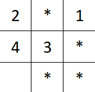
\includegraphics[width=0.3\textwidth]{assets/q6-a1.png}
          \end{minipage}
          \hfill
          \begin{minipage}{0.45\textwidth}
            \centering
            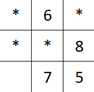
\includegraphics[width=0.3\textwidth]{assets/q6-a2.png}
          \end{minipage}
        \end{figure}

    \item چهار پازل 1 تا 4 نگه داشته می‌شوند و باقی پازل‌ها حذف می‌شوند، به همین ترتیب برای چهار پازل 5 تا 8.
        \begin{figure}[h]
          \centering
          \begin{minipage}{0.45\textwidth}
            \centering
            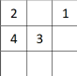
\includegraphics[width=0.3\textwidth]{assets/q6-b1.png}
          \end{minipage}
          \hfill
          \begin{minipage}{0.45\textwidth}
            \centering
            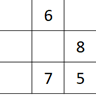
\includegraphics[width=0.3\textwidth]{assets/q6-b2.png}
          \end{minipage}
        \end{figure}
\end{enumerate}

\bigskip
\rule{\linewidth}{0.4pt}

\section{سوال هفتم}
مسئلۀ زیر را بخوانید و به سوالات پاسخ دهید:

یک رودخانه دو خشکی را از هم جدا کرده است. در سمت چپ آن 3 گرگ و 3 اسب قرار دارند. هدف این است تا با یک قایق 2 نفره تمام آنها را به سمت راست رودخانه منتقل کرد، بطوری که هیچگاه در خشکی‌ها تعداد گرگ‌ها از اسب‌ها بیشتر نباشد (در صورتی که اسبی در آن خشکی وجود داشته باشد). هزینه هر جابجایی قایق برابر 1 واحد است. هر گره را بصورت $\langle H,W,B\rangle$ در نظر بگیرید که $H$ تعداد اسب‌ها و $W$ تعداد گرگ‌ها در سمت چپ و $B$ راست یا چپ بودن قایق را نشان می‌دهد.

\begin{enumerate}[label=\alph*-]
    \item یک \emph{Problem Relaxed} برای مسئله بنویسید.
    \item بر مبنای مسئلۀ Relaxed شده در قسمت «الف»، یک هیوریستیک قابل قبول طرح کنید. (هیوریستیک باید تابعی از یک متغیر باشد و نباید تابع ثابت باشد.)
    \item یکنواخت بودن یا نبودن هیوریستیک خود را نشان دهید. (راهنمایی: تمام حالات حرکت را برای شرط یکنواخت بودن در نظر بگیرید.)
\end{enumerate}

% در صورت نیاز به نمودار فضای حالت یا گراف، اینجا قرار دهید:
% \begin{center}
%   \includegraphics[width=0.7\textwidth]{assets/q7-graph.png}
% \end{center}

\bigskip
\rule{\linewidth}{0.4pt}

% Add more sections as needed...

\end{document}
